\section{HMM and sparsity}
It is our experience that when using a \gls{hmm} to model real world processes, the transition matrix often becomes sparse due to the nature of the process modeled.
For example, in human trait recognition, a \gls{hmm} can be used to model the motion of a particular person while he walks\cite{trait-recognition}.
If focusing on the lower part of the body, consider one state that represents the longest gap between the two feet while walking, where the right foot is in front. It is natural that this state cannot directly lead to the opposite state where the left foot is in front. There has to be a number of intermediate states to represent a more fluid movement, and hence the transition matrix may be quite sparse \gls{hmm}.

When building a system to recognize handwritten text, the transitions matrix of a \gls{hmm} can capture the probability of seeing a particular letter given a letter that precedes it.
In the English language (and possible many other languages), there are many instances of two particular letters, that very rarely or never occur next to each other. An example of the transition probabilities between letters in the English alphabet can be seen in figure \ref{fig:ocr-transitions}, which was made from an analysis of 6020 handwritten words provided by Rob Kassel at MIT Spoken Language Systems Group\cite{thomas-letter-pair-analysis-picture}. Visually, it seems like the transition matrix has many probabilities of zero or very close to. The handouts\cite{leon-letter-pair-analysis-handouts} of Jeffrey S. Leon, confirms the many zero values by providing specific number of occurrences based on analysis of seven English language novels.
\begin{figure}
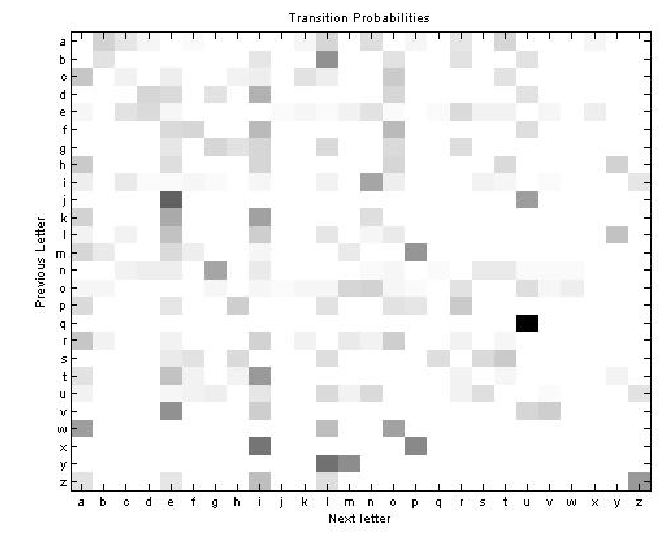
\includegraphics[scale=0.4]{pictures/ocr-transitions.jpg}
\label{fig:ocr-transitions}
\caption{The transition probabilities between two letters in an English word. White colour denotes a probability of 0 while black denotes a probability of 1.}
\end{figure}